%%
%% This is file `mcmthesis-demo.tex',
%% generated with the docstrip utility.
%%
%% The original source files were:
%%
%% mcmthesis.dtx  (with options: `demo')
%% !Mode:: "TeX:UTF-8"
%% -----------------------------------
%%
%% This is a generated file.
%%
%% Copyright (C)
%%     2010 -- 2015 by latexstudio
%%     2014 -- 2016 by Liam Huang
%%     2014 -- 2016 by latexstudio.net
%%
%% This work may be distributed and/or modified under the
%% conditions of the LaTeX Project Public License, either version 1.3
%% of this license or (at your option) any later version.
%% The latest version of this license is in
%%   http://www.latex-project.org/lppl.txt
%% and version 1.3 or later is part of all distributions of LaTeX
%% version 2005/12/01 or later.
%%
%% This work has the LPPL maintenance status `maintained'.
%%
%% The Current Maintainer of this work is Liam Huang.
%%
\documentclass{mcmthesis}
\mcmsetup{CTeX = false,   % 使用 CTeX 套装时,设置为 true
        tcn = 2010755, problem = A,% 队伍控制号码,接受一个字符串作为值;选题,接受一个字符串作为值;
        sheet = false, %为真时将输出摘要页,否则不输出;默认为 true。
        color = red,  %设置控制页的题目号的颜色
        titleinsheet = true, %为真时将在摘要页输出标题,否则不输出;默认为 false。
        keywordsinsheet = true,%为真时将在摘要页输出关键字,否则不输出;默认为 false。
        titlepage = false,%为真时将输出标题页,否则不输出;默认为 true。
        abstract = true}%为真时将在标题页输出摘要和关键词,否则不输出;默认值为 true。
\usepackage{palatino}  %控制正文字体,若是不喜欢可以注释掉。
\usepackage{lipsum}
\usepackage{tikz}
\usepackage{xcolor}
\usepackage{verbatim}
\usepackage{subfigure} 
\usetikzlibrary{arrows,shapes,chains}
\title{Title!}
\author{\url{http://www.latexstudio.net}\\[3pt]  \href{http://www.latexstudio.net/}
  {\includegraphics[width=7cm]{mcmthesis-logo}}}
\date{\today}

\makeatletter
\renewcommand*\l@section{\@dottedtocline{1}{12pt}{12pt}}
\makeatother

%%%%%%%%%%%%%%%%%%%%%%%%%%%%%%%%%%%%%%%%
%% MCM/ICM LaTeX Template %%
%% 2020 MCM/ICM           %%
%%%%%%%%%%%%%%%%%%%%%%%%%%%%%%%%%%%%%%%%
\usepackage{geometry}
\geometry{left=1in,right=0.75in,top=1in,bottom=1in}

%%%%%%%%%%%%%%%%%%%%%%%%%%%%%%%%%%%%%%%%
% Replace ABCDEF in the next line with your chosen problem
% and replace 1111111 with your Team Control Number
\newcommand{\Problem}{A}
\newcommand{\Team}{\# 2010755}
%%%%%%%%%%%%%%%%%%%%%%%%%%%%%%%%%%%%%%%%

\usepackage{newtxtext}
\usepackage{amsmath,amssymb,amsthm}
\usepackage{newtxmath} % must come after amsXXX

%\usepackage[pdftex]{graphicx}

\usepackage{fancyhdr}
\lhead{Team \Team}
\rhead{}
\cfoot{}

\newtheorem{theorem}{Theorem}
\newtheorem{corollary}[theorem]{Corollary}
\newtheorem{lemma}[theorem]{Lemma}
\newtheorem{definition}{Definition}

%%%%%%%%%%%%%%%%%%%%%%%%%%%%%%%%
\begin{document}
\graphicspath{{.}}  % Place your graphic files in the same directory as your main document
\DeclareGraphicsExtensions{.pdf, .jpg, .tif, .png}
\thispagestyle{empty}
\vspace*{-16ex}
\centerline{\begin{tabular}{*3{c}}
	\parbox[t]{0.3\linewidth}{\begin{center}\textbf{Problem Chosen}\\ \Large \textcolor{red}{\Problem}\end{center}}
	& \parbox[t]{0.3\linewidth}{\begin{center}\textbf{2020\\ MCM/ICM\\ Summary Sheet}\end{center}}
	& \parbox[t]{0.3\linewidth}{\begin{center}\textbf{Team Control Number}\\ \Large \textcolor{red}{\Team}\end{center}}	\\
	\hline
\end{tabular}}
\begin{Huge}
\begin{center}
\textbf{XXX}
\end{center}
\end{Huge}
%%%%%%%%%%% Begin Summary %%%%%%%%%%%
% Enter your summary here replacing the (red) text
% Replace the text from here ...
\begin{center}
\begin{large}
\textbf{Summary}
\end{large}
\end{center}



% to here
%%%%%%%%%%% End Summary %%%%%%%%%%%

%%%%%%%%%%%%%%%%%%%%%%%%%%%%%%
\clearpage
\pagestyle{fancy}

% Uncomment the next line to generate a Table of Contents
%\tableofcontents 

\setcounter{page}{1}
\rhead{Page \thepage\ of \pageref{LastPage}}
%%%%%%%%%%%%%%%%%%%%%%%%%%%%%%


\begin{abstract}
Firstly,\cite{1}

Secondly,

Thirdly,

We then

Finally,

\begin{keywords}
Generalized Additive Model, Markov model
\end{keywords}
\end{abstract}
\maketitle

\tableofcontents


\section{Introduction}




\section{Assumption}

There are some symbols appear in the model. We show them below:
\begin{table}[htbp]
\centering
\caption{Symbols in Chapter 3}
\begin{tabular}{cp{0.8\textwidth}}
\toprule
 Symbols & Description\\
\midrule
 $i$ & Station variable \\
 $DS_i$ & Density of fish( mackerel or herring) at station i $(kg/km^2)$\\
 $H_i$ & Horizontal opening of trawl at station i  $(km)$\\
 $TD_i$ & Distance of the trawl haul $(km^2)$ \\
 $C_i$ &  Catch at station i$(kg)$\\

  $\lambda_i$ &   Longitude at station i $(^\circ W)$\\
 $\phi_i$ &   Latitude at station i $(^\circ N)$\\
$SST_i$ &  Sea Surface Temperature at station i $(^\circ C)$\\

 $z_i$ & Zooplankton's dry weight at station i $(kg)$\\
 $SSB_i$ &  Spawning-stock biomass at station i \\
  $b_i$ & Number of biological species at station i\\
$y$ & Year \\
$j$& Rectangular number\\
$t$ & Time  \\
$M_j(t)$ & State of the $j_{th}$ rectangle at time $t$ \\
$P_{M_w,M_k}$ &  Transition probability for the State $M_w$changing into State $M_k$\\
\bottomrule
\end{tabular}
\end{table}


\begin{table}[htbp]
\centering
\caption{Symbols in Chapter 4}
\begin{tabular}{cp{0.8\textwidth}}
\toprule
 Symbols & Description\\
\midrule
$B$ &  Backshift operator\\

\bottomrule
\end{tabular}
\end{table}
\begin{table}[htbp]
\centering
\caption{Symbols in Chapter 5 \& 6}
\begin{tabular}{cp{0.8\textwidth}}
\toprule
 Symbols & Description\\
\midrule
 %\rowcolor{lightgray}
$CPUE_{y}$ & Catch Per Unit Effort in year $y$\\

\bottomrule
\end{tabular}
\end{table}





\section{Data preprocessing and Descriptive statistics }
\subsection{Data preprocessing}
For data preprocessing on the data provided by Sunshine company, our team mainly considers
two aspects. The first is the removal of useless data, and the second is the quantification of text data.

\subsubsection{Removal of meaningless data}

By observing the data given in the question, we find that there is a lot of irrelevant data. First, remove fields that are not relevant to the data analysis, such as "marketplace","customer\_id","review\_id",

"product\_id","product\_category"
We remove extranical product evaluations in the dataset, such as the product evaluations for pillow driers in the baby pacifier product evaluation dataset. We also found that there were a lot of user comments that were meaningless, and we culled them out.

\subsubsection{Data type conversion}

The data marks "N" and "Y" are converted to "0" and "1", and the string data is converted to floating point numbers, which is convenient for the next statistical analysis and prediction.

\section{The relationship between star rating and review text based
on Logistic Regreesion}

\subsection{Quantification of review text based on TF-IDF Method}
Now, we want to research the relationship between reviews and star rating. Generally
speaking, the more positive the comment is, the higher the star rating will be, and the lower
the star rating is, the more negative the comment will be. 

On the one hand, we verify whether
this conclusion is valid. On the other hand, we want to understand the features that people
who give good reviews are more interested in and what features that people who give bad
reviews complain about most. In order to achieve this purpose, we use TF-IDF technology
to quantize review according to its importance in all reviews.

We concatenated the "review\_headline" with the "review\_body" and removed extraneous punctuation. Then we uniformly convert the letters to lowercase and use the spaCy method to convert the word into its root form, which is convenient for subsequent text analysis.

Then, deal with the data of
star rating. We denote ’one star’,’two star’ , ’three star’ as 0 (negative), and others as 1 (positive). Thus we gain
a series data of 0-1 from star rating data. After that, we get some words that have a great
influence on consumers’ attitude through logistic regression between the above 0-1 series and
those quantified review.Thereupon, some product features consumers interested in most can
be concluded, which Sunshine Company need to track once their three products are placed on
sale in the online marketplace.

TF-IDF is a statistical method to reflect the how important a word is to a document in a
collection or corpus.The following is TF-IDF formula:

\begin{equation}
tf - idf(t,d)=tf(t,d) \times idf(t)
\end{equation}
\begin{equation}
tf(t,d)=\frac{n(t,d)}{\sum_k{n_{k,d}}}
\end{equation}
\begin{equation}
idf(t,d)=log(\frac{n_d}{df(d,t)})+1
\end{equation}

$tf(t, d)$ is tf value, indicating the frequency fo term t in a text d.

$idf(t)$ is the calculation formula of idf value of term t; nd is the number of text in training set;

$df(d, t)$ is the total number of documents containing term t. The idf value is an improvement
of word weight, not only considering the frequency of words in the text, but also the frequency
of words in the general text. 

To avoid 0 occurring in the denominator, the formula of idf we actually use is
\begin{equation}
idf(t)=log(\frac{1+n_d}{1+df(d,t)})+1
\end{equation}
\subsection{Model Comparison}

We labeled reviews with a score greater than 3 as 1 (positive), and those with a score less than 3 as 0 (negative).

We use the method of TF-IDF word vector to vectorize the text.

We first vectorize the text using the sklearn library's method of generating TF-IDF word vectors.

Using positive/negative tags, we use Bernoulli Naive Bayes classifier, Multinomial Naive Bayes classifier, Support Vector Machine(SVM) ,Stochastic gradient descent Classifier(SGD Classifier) and Logistic Regression model for text sentiment analysis.
Then, we evaluated the fitting effects of the five models using four indexes, namely precision rate, recall rate, F1 measurement and ROC curve.

By comparison, the logistic regression model is the best.

\begin{enumerate}[*]
\item Precision rate: As can be seen from the following table, the accuracy rate of Logistic Regression model is as high as 89\%.

\begin{center}
\textbf{The precision rate of each classifier}
\begin{tabular}{|c|c|c|c|c|c|}
\hline
\makebox[0.12\textwidth][c] {Classifier}& \makebox[0.18\textwidth][c] {Logistic Regression}& \makebox[0.16\textwidth][c] {SGD Classifier}& \makebox[0.08\textwidth][c] {SVM}& \makebox[0.12\textwidth][c] {Bernoulli BN}& \makebox[0.15\textwidth][c] {Multinomial BN} \\ \hline
Precision rate    &0.89276 &0.89186 &0.87873  &0.84027 &0.83077	\\ \hline 
\end{tabular}
\end{center}
\item Recall,f1-score measurements and metrics
It can be seen from the ~\autoref{fig:anna1} that the recall rates of SGD Classifier, logistic regression model and support vector machine are almost the same, while the F1 score of logistic regression model is higher, indicating that the logistic regression model has better performance.
\item ROC curve: AUC (Area Under Curve) is defined as the Area Under the ROC Curve. In many cases, the ROC curve cannot clearly indicate which classifier has better effect, so we use AUC value as the evaluation criterion of the model: classifier with larger AUC has better effect.The result is shown in ~\autoref{fig:anna2} .

\begin{figure}[htbp]
\centering
\begin{minipage}[t]{0.48\textwidth}
\centering
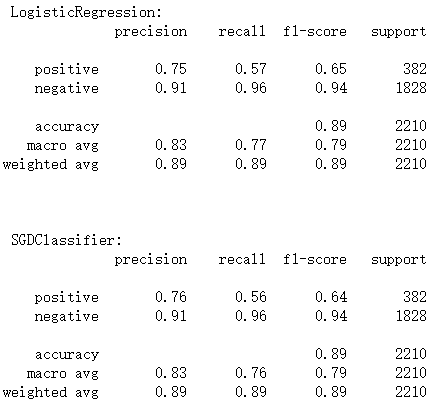
\includegraphics[width=8cm]{./figures/f1.png}
\caption{Classifiers comparision with recall rates and f1-score}
\label{fig:anna1}
\end{minipage}
\begin{minipage}[t]{0.48\textwidth}
\centering
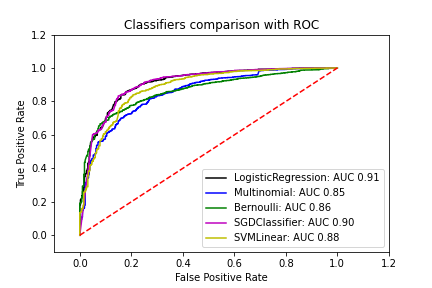
\includegraphics[width=9cm]{./figures/f2.png}
\caption{Classifiers comparision with ROC}
\label{fig:anna2}
\end{minipage}
\end{figure}
\end{enumerate}






\subsection{Logistic Regression}

Logistic regression is a classification model,whose principle is as follows.

For a given training data set,$T = {(x_1, y_1),(x_2, y_2), ...,(x_n, y_n)}$.

Among them,$x_i \in R^n,y_i \in {0, 1}$Assume$ z = -(wx + b)$.Then we call the following probability distribution logistic
regression model:

\begin{equation}
P(Y=0|x)=\frac1{1+e^{-z}}=\frac1{1+e^{wx+b}}
\end{equation}
\begin{equation}
P(Y=1|x)=1-\frac1{1+e^{-z}}=\frac{e^{-z}}{1+e^{-z}}=\frac{e^{wx+b}}{1+e^{wx+b}}
\end{equation}
In the equation above ,we call the $\omega$ the weight coefficient.To facilitate the representation
of multiple variables,let’s introduce the weight coefficent vector $W = (w1, w2, ..., wn, b)'$ .The sample vector$ X = (x1, x2, ..., xn, 1)'$.Now,the matrix of logistic regression is represented as follows.
\begin{equation}
P(Y=0|x)=\frac1{1+e^{WX}}
\end{equation}
\begin{equation}
P(Y=1|x)=\frac{e^{WX}}{1+e^{WX}}
\end{equation}
In this model, we need to estimate the weight coefficient vector$ W$.The method of estimation
is maximum likelihood estimation(MLE).
We assume:
\begin{equation}
P(Y=1|x)=\pi(x)
\end{equation}
\begin{equation}
P(Y=0|x)=1-\pi(x)
\end{equation}

The logarithmic likelihood function
\begin{equation}
L(W)=\sum^n_{i=1}(y_ilog(\pi(x_i)))+(1-y_i)log(1-\pi(x_i))
\end{equation}
\begin{equation}
L(W)=\sum^n_{i=1}(y_ilog(\frac{\pi(x_i)}{1-\pi(x_i)}))+log(1-\pi(x_i))
\end{equation}
\begin{equation}
L(W)=\sum^n_{i=1}(y_i(w_ix_i-log(1+e^{w_i*x_i})))
\end{equation}

Let $\frac{\partial L}{\partial w_i}=0$, We can get the maximum of the likelihood function.The vector $\hat W$ that we get
from that is the maximum likelihood estimation of the weight parameter.According to statistical study, maximum likelihood estimation has good statistical properties.So we now have a logistic
regression estimation model as follows:

\begin{equation}
P(Y=0|x)=\frac1{1+e^{\hat WX}}
\end{equation}
\begin{equation}
P(Y=1|x)=\frac{e^{\hat WX}}{1+e^{\hat WX}}
\end{equation}

\subsection{The result of Regression}
Previously, we have introduced the TF IDF algorithm to deal with the word frequency of
text. We applied this algorithm to the comments of three products and took the data obtained
as the independent variable of logistic regression. For example, in the hair dryer product, we
extract words such as ” quiet,spark’ in user comments as independent variables, and the value
of independent variables is obtained by the TF IDF algorithm above.As for the treatment of
dependent variables ,we denote ’one star’,’two star’ , ’three star’ as 0, and others as 1.

The training sets of the obtained independent variables and dependent variables are carried
out logistic regression.We used test sets to verify the accuracy of the model. The overall
regression results of the three products and their accuracy are shown in ~\autoref{tab2}.


\begin{table}[h]
\centering
\caption{Logistic regression accuracy results}
\begin{tabular}{ccccc}
\toprule[1.5pt]
\makebox[0.12\textwidth][c] {}& \makebox[0.15\textwidth][c] {features}& \makebox[0.15\textwidth][c] {train records}& \makebox[0.15\textwidth][c] {test records}& \makebox[0.15\textwidth][c] {Model Accuracy} \\ \hline
hairdryer    &156971 &8602 &2868  &0.88479\\ 
microwave    &51778 &1211 &404  &0.87227\\ 
pacifier    &251940 &14204 &4735  &0.89276\\ 
\toprule[1.5pt]
\end{tabular}
\label{tab2}    
\end{table}

According to the above table, the accuracy of logistic regression estimation of the three
products is above 80\%, so it can be considered that the results of logistic regression estimation
are statistically satisfactory.
Next, we will show the coefficient estimation obtained by logistic regression and its specific
meaning.Since there are too many independent variables in logistic regression to show them
all, we only show some representative variables in the following table.



The specific meaning of the coefficient of the variable obtained by logistic regression is the
influence of the word frequency of the variable appearing in the comment on the star rating.If
the variable is a more positive term, the coefficient is positive and larger,if the variable is a more
negative term, the coefficient is negative and smaller.According to this principle, combined with
the results obtained in the above table, we can find the following rules.
People generally like the heat setting in the hair dryer, and some hair dryers has the advantages
of fast, light, small sound and so on. Among them, heat setting is the most attractive.But
some brands of hair dryer and there will be sparks, too hot, too heavy, too loud and other
shortcomings.We can see that customers are very concerned about the temperature and lightness
of the hair dryer.
Customers generally concern about the advantage of microwave oven,which is simple,
occupying small space , clean and the low price.But the whirlpool microwave got a lot of bad
reviews, and users hated the constant need for repairs and worried about its quality.
In the eyes of customers, the pacifier is a perfect gift, soft but tough, and very cute.However,
some customers think that the price of pacifier is too high, some of the quality of the pacifier is
very poor.Even some customers hate pink pacifiers.


\section{Strengths and Weaknesses}
\subsection{Strengths}



\subsection{Weaknesses}


\section{A Letter}
\textbf{MEMORANDUM}~\\
\textbf{TO: Hook Line and Sinker}\\
\textbf{FROM:Team \#2010755}\\


\begin{thebibliography}{99}
\bibitem{1} Olafsdottir, A. H., Utne, K. R., Jacobsen, J. A., Jansen, T., Óskarsson, G. J., Nøttestad, L., ... \& Slotte, A. (2019). Geographical expansion of Northeast Atlantic mackerel (Scomber scombrus) in the Nordic Seas from 2007 to 2016 was primarily driven by stock size and constrained by low temperatures. Deep Sea Research Part II: Topical Studies in Oceanography, 159, 152-168.
\bibitem{2}  Wu shengnan, Chen xinjun, \& liu zhonan. (2019). Prediction model of Japanese mackerel resource abundance in the northwest Pacific based on GAM. Acta oceanologica sinica, 41(8), 36-42.
\bibitem{3}\url{http://ecosystemdata.ices.dk/Map/index.aspx?Action=AddLayer&TAXA=6799&YEAR=2017&Grid=-1&Color=random&Type=Count}
\bibitem{4} Nøttestad, L., Anthonypillai, V., Tangen, Ø., Høines, A., Utne, K. R., Oskarsson, G. J., ... \& Jansen, T. (2016). Cruise report from the International Ecosystem Summer Survey in the Nordic Seas (IESSNS) with M/V M. Ytterstad’, M/V ‘Vendla’, M/V ‘Tróndur ı Gøtu’, M/V ‘Finnur Frıði’and R/V ‘Arni Friðriksson, 1-31.
\bibitem{5} Zhang yunquan, zhu yaohui, li cunlu, feng renjie, \& ma lu. (2015). Implementation of generalized additive model in R software. China health statistics, 32(6), 1073-1075.
\bibitem{6}Li dewei, zhang long, wang Yang, \& zhu wenbin. (2015). Analysis of the relationship between CPUE and environmental factors in Argentine sliders based on GAM. Fisheries modernization, (2015 04), 56-61.
\bibitem{7}XiaoXin Han(2009). Research on the Contribution Rates of Three Industries in
China Based on Markov Chain. Cooperative Economy \& Science (15), 24-25.
\bibitem{8}Chang, X., Gao, M., Wang, Y., \& Hou, X. (2012). Seasonal autoregressive integrated moving average model for precipitation time series. Journal of Mathematics \& Statistics, 8(4).
\bibitem{9}
Akaike H. (1987) Factor Analysis and AIC. In: Parzen E., Tanabe K., Kitagawa G. (eds) Selected Papers of Hirotugu Akaike. Springer Series in Statistics (Perspectives in Statistics). Springer, New York, NY
\end{thebibliography}

\begin{appendices}

\section{First appendix}

\end{appendices}

\end{document}

%%
%% This work consists of these files mcmthesis.dtx,
%%                                   figures/ and
%%                                   code/,
%% and the derived files             mcmthesis.cls,
%%                                   mcmthesis-demo.tex,
%%                                   README,
%%                                   LICENSE,
%%                                   mcmthesis.pdf and
%%                                   mcmthesis-demo.pdf.
%%
%% End of file `mcmthesis-demo.tex'.

\end




